\documentclass[11pt]{beamer}
\usepackage[utf8]{inputenc}
\usetheme{Boadilla}
\setbeamertemplate{navigation symbols}{}
\usepackage{lmodern}
\usepackage[T2A]{fontenc}
\usepackage{cmbright}
\usepackage[russian]{babel}
\usepackage{subcaption}
%\usetheme{Darmstadt}

\usetheme{Boadilla}
\setbeamertemplate{navigation symbols}{}

\usepackage{amsmath}
\usepackage{amsfonts}
\usepackage{bm}
\usepackage{graphicx}
%\usepackage[usenames]{color}
\usepackage{colortbl}
% Использовать полужирное начертание для векторов
\let\vec=\mathbf

\DeclareMathOperator{\mathspan}{span}
\DeclareMathOperator{\mathdim}{dim}
\DeclareMathOperator{\rank}{rank}
\DeclareMathOperator{\diag}{diag}

\newcommand\eqdef{\mathrel{\stackrel{\makebox[0pt]{\mbox{\normalfont\tiny def}}}{=}}}

\begin{document}
	\author{Кононыхин Иван Александрович}
	
	\title[]{Научная и компьютерная коммуникация в современных условиях}
	\subtitle{<<Обнаружение разладки с помощью метода SSA>>}
	%\logo{}
	\institute[]{
		группа 20.М03-мм\\
		Санкт-Петербургский государственный университет\\
		Прикладная математика и информатика
	}
	\date{\number\year}
	\setbeamercovered{transparent}
	\setbeamertemplate{navigation symbols}{}
	\begin{frame}[plain]
		\maketitle 
	\end{frame}
	
	\begin{frame}
		\centering
		Введение в теорию
	\end{frame}
	
	\begin{frame}
		\frametitle{Основные обозначения}
		\begin{block}{Обозначения}
			$F^{(1)} = F_{N_1}^{(1)}$, $F^{(2)} = F_{N_2}^{(2)}$ - временные ряды.
			
			$L: 2 \leq L \leq \min(N_1 - 1, N_2)$ - длина окна.
			
			$ U_l^{(1)}, l = 1, \dotsc, L $ --- собственные векторы траекторной матрицы ряда $ F^{(1)} $
			
			$\mathfrak{L}^{(L, 1)}$ --- линейное пространство, натянутое на $L$---сдвинутые векторы ряда $F^{(1)}$, $ d \eqdef dim \; \mathfrak{L}^{(L, 1)} $
			
			$ I = \{i_1, \dotsc, i_r\} $ --- подмножество $ \{1, \dotsc, L\} $
			
			$ \mathfrak{L}_r^{(1)} \eqdef span(U_l^{(1)}, l \in I) $
			
			$ X_1^{(2)}, \dotsc, X_{K_2}^{(2)} $ --- $L$-сдвинутые векторы ряда $F^{(2)} $
		\end{block}
	\end{frame}
	
	\begin{frame}
		\frametitle{Индекс неоднородности}	
		\begin{block}{Определение}  \textit{Индекс неоднородности}:
			$$ g(F^{(1)}; F^{(2)}) = \frac{\sum\limits_{l=1}^{K_2}\mathrm{dist}^2(X_l^{(2)}, \mathfrak{L}_r^{(1)})}{\sum\limits_{l=1}^{K_2}\|X_l^{(2)}\|^2} = \frac{\sum\limits_{l=1}^{K_2}\;(\|X_l^{(2)}\|^2 - \sum\limits_{i=1}^{r}\langle X_l^{(2)}, U_i^{(1)}\rangle^2)}{\sum\limits_{l=1}^{K_2}\|X_l^{(2)}\|^2} = $$
			$$ = 1 - \frac{\sum\limits_{l=1}^{K_2}\;\sum\limits_{i=1}^{r}\langle X_l^{(2)}, U_i^{(1)}\rangle^2}{\sum\limits_{l=1}^{K_2}\|X_l^{(2)}\|^2}. $$
		\end{block}
		Индекс неоднородности характеризует несоответствие между рядом $F^{(2)}$ и структурой ряда $F^{(1)}$ (описываемого подпространством $ \mathfrak{L}_r^{(1)} $).
		
		$g \in [0, 1]$.
		
	\end{frame}
	\begin{frame}
		\frametitle{Обозначения}
		\begin{block}{}
			$ F_N: F_N = (f_0, \dotsc, f_{N - 1}), N > 2 $ --- исходный временной ряд;
			
			$ F_{i, j} $ --- подряды ряда $ F_N: F_{i, j} = (f_{i}, \dotsc, f_{j}), \; 0 \leq i < j \leq N - 1 $;
			
			$ B $ --- длина базовых подрядов ряда $ F_N: B > L $;
						
			$ T $ --- длина тестовых подрядов ряда $ F_N: T \geq L $;
			
			
			$ F_{i, i+B-1} $ --- Базовый подряд.
			
			$ F_{j, j+T-1} $ --- Тестовый подряд.

		\end{block}
	\end{frame}

	\begin{frame}
		\frametitle{Строковая функция обнаружения неоднородности}
		\begin{block}{Определение}
			Ряд $ D_{T,N}^{(r)} $, элементы которого задаются как 
			$$ d_{n-1}^{(r)} \eqdef g(F_{1, B};\; F_{n-T+1, n}), \;\; T \leq n \leq N. $$
			есть \textbf{строковая функция обнаружения}.
		\end{block}
	\end{frame}
	
	\begin{frame}
		\centering
		Аналитическая оценка индекса неоднородности при изменении частоты гармоники
	\end{frame}
	
	\begin{frame}
		\frametitle{Постановка задачи}
		\begin{block}{Задача}
			Попробуем аналитически упростить индекс неоднородности $ g $, чтобы явно увидеть, как разности частот ряда до и после разладки влияют на его значения.
		\end{block}
		Рассмотрим ряд
		\begin{equation*} 
			F_N = 
			\begin{cases} 
				C_1\sin(2\pi\omega_1 n + \phi_1),\ n \in [0, Q-1], \\ 
				C_2\sin(2\pi\omega_2 n + \phi_2),\ n \in [Q, N-1]. 
			\end{cases} 
		\end{equation*} 
		Пусть $ \omega_1 \neq \omega_2;\; C_1 = C_2 $. Для простоты зададим амплитуды $ C_1 = C_2 = 1 $.
	\end{frame}
	
	
	\begin{frame}
		\frametitle{Индекс неоднородности}
		$$ g(F^{(1)}; F^{(2)}) = \frac{\sum\limits_{l=1}^{K_2}\mathrm{dist}^2(X_l^{(2)}, \mathfrak{L}_r^{(1)})}{\sum\limits_{l=1}^{K_2}\|X_l^{(2)}\|^2} = \frac{\sum\limits_{l=1}^{K_2}\;(\|X_l^{(2)}\|^2 - \sum\limits_{i=1}^{r}\langle X_l^{(2)}, U_i^{(1)}\rangle^2)}{\sum\limits_{l=1}^{K_2}\|X_l^{(2)}\|^2} = $$
		$$ = 1 - \frac{\sum\limits_{l=1}^{K_2}\;\sum\limits_{i=1}^{r}\langle X_l^{(2)}, U_i^{(1)}\rangle^2}{\sum\limits_{l=1}^{K_2}\|X_l^{(2)}\|^2}. $$
	\end{frame}
	
	\begin{frame}
		\frametitle{Индекс неоднородности: аппроксимация}
		Пусть $ F^{(1)} $ - часть ряда $ F_N $ при $ n < Q $, а $ F^{(2)} $, при $ n >= Q $.
				
		\begin{figure}[b]
			\centering
			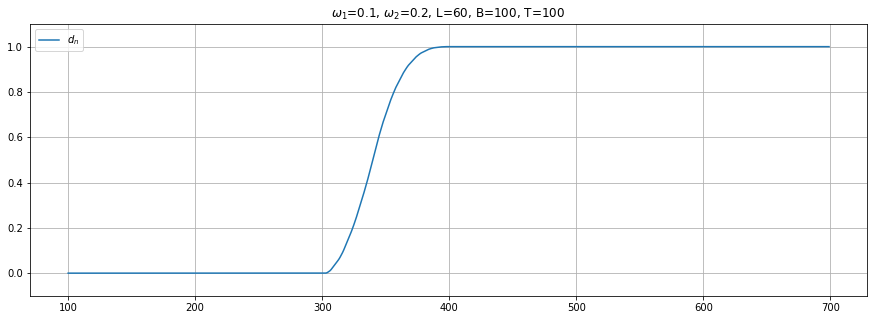
\includegraphics[width=0.75\linewidth]{imgs/heterogeneity_index_row.png}
		\end{figure}
		\small
		$$ g(F^{(1)}; F^{(2)}) = 1 - \frac{\sum\limits_{l=0}^{K_2-1}\;\sum\limits_{i=0}^{r-1}\langle X_l^{(2)}, U_i^{(1)}\rangle^2}{\sum\limits_{l=0}^{K_2-1}\|X_l^{(2)}\|^2} \approx $$
		$$ 1 - \frac{\left[ \left(  \frac{\sin(2\pi Lb)}{4\pi b} - \frac{\sin(2\pi La)}{4\pi a}   \right)^2 + \left(  \frac{\cos(2\pi Lb) - 1}{4\pi b} - \frac{\cos(2\pi La) - 1}{4\pi a}  \right)^2 \right]}{\frac{L^2}{4}} = g_a(\omega_1, \omega_2),$$
		где $ a = \omega_1 + \omega_2, b = \omega_1 - \omega_2 $.
	\end{frame}
	
	\begin{frame}
		\frametitle{Проверка точности аппроксимации: изменения $ L $}
		Зададим параметры:
		
		$ N = 700,\; Q = 301,\; B = 200,\; T = 200 $
		
		Зафиксируем частоты и будем изменять $ L $.
		
		\begin{figure}[b]
			\centering
			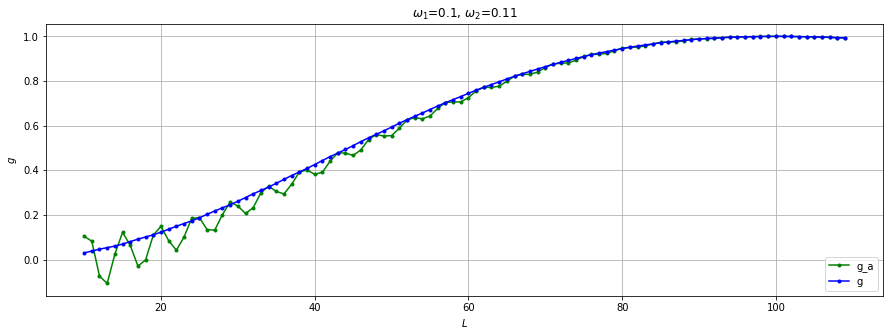
\includegraphics[width=0.6\linewidth]{imgs/dynamics_L}
		\end{figure}
		
		\begin{figure}[b]
			\centering
			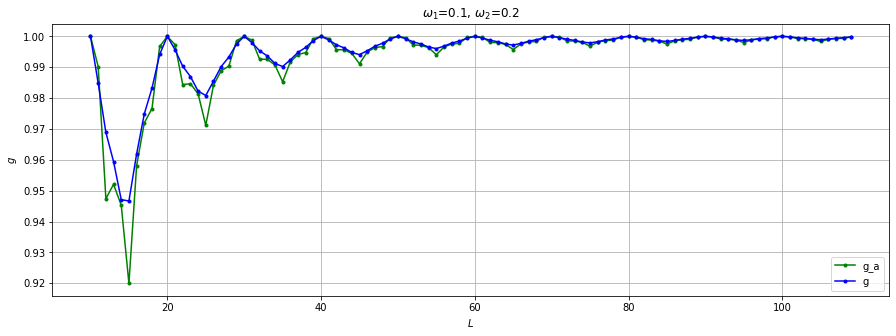
\includegraphics[width=0.6\linewidth]{imgs/dynamics_L_1}
		\end{figure}
		
	\end{frame}
	
	\begin{frame}
		\centering
		Система обнаружения структурной неоднородности ряда с автоматически выстраиваемым порогом срабатывания на основе выведенной аналитической формулы.
	\end{frame}
	
	\begin{frame}
		\frametitle{Постановка задачи}
		Рассмотрим ряд 
		\begin{equation*} 
			F_N = 
			\begin{cases} 
				C\sin(2\pi\omega_1 n + \phi_1),\ n \in [0, Q-1], \\ 
				C\sin(2\pi\omega_2 n + \phi_2),\ n \in [Q, N-1], 
			\end{cases} 
		\end{equation*}
		где $ Q $ --- момент возмущения. 
		
		
		Система: 
		
		\begin{itemize}
			\item Вход:
			\begin{enumerate}
				\item $ F_N $;
				\item $ k $ --- длина интервала, за который нужно определить момент возмущения $ \hat{Q} $.
			\end{enumerate}
			\item Выход:
			\begin{enumerate}
				\item $ \hat{Q} $ --- момент обнаружения неоднородности.
			\end{enumerate}
			\item Алгоритм:
			\begin{enumerate}
				\item Вычисляем порог $ \gamma $;
				\item Определяем $ \hat{Q} $ как преодоление порога $ \gamma $ кривой $ d_n $.
			\end{enumerate}
		\end{itemize}
		Задача:
		
		Выбрать порог $ \gamma $ так, чтобы $ \hat{Q} \in [Q, Q+k] $.
	\end{frame}
	
	\begin{frame}
		\frametitle{Оценка $ \gamma $}
		В качестве верхней границы $ \gamma $ можно взять значение переходного интервала в точке $ k $.
		
		При добавлении шума с дисперсией $ \sigma^2 $ строковая функция неоднородности $ d_n $ до разладки смещается от $ 0 $. Если взять слишком маленькое значение $ \gamma $, $ \hat{Q} < Q $, поэтому нижняя граница зависит от дисперсии шума $ \sigma^2 $.
		
		Для таких рядов надо либо знать $ \sigma^2 $, либо иметь данные для оценки значений $ d_n $ где точно отсутствует неоднородность. 
		
		\begin{figure}[b]
			\centering
			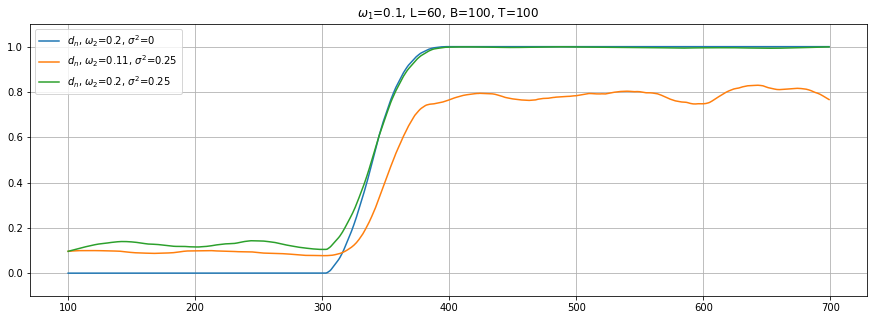
\includegraphics[width=\linewidth]{imgs/estimate_gamma_noise}
		\end{figure}
	\end{frame}

	\begin{frame}
		\frametitle{Оценка $ \gamma $: нижняя граница}
		Предположим, у нас есть нужные данные и мы смогли оценить нижнюю границу $ \gamma = \gamma_{min} $.
		
		\bigskip
		Если мы знаем $ \sigma^2 $, то $ \gamma_{min} \approx \frac{\sigma^2}{C^2/2+\sigma^2} $.
		
		\begin{figure}[b]
			\centering
			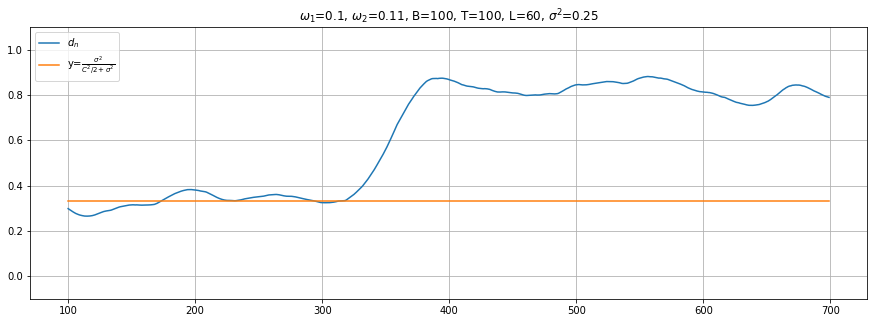
\includegraphics[width=\linewidth]{imgs/estimate_noise}
		\end{figure}
		
	\end{frame}

	\begin{frame}
		\frametitle{Оценка $ \gamma $: верхняя граница}
		Для определения верхней границы $ \gamma $ мы можем воспользоваться аналитической аппроксимацией $ g_a(\omega_1, \omega_2) $, однако для этого нам нужно знать частоты до и после разладки.
	\end{frame}

	\begin{frame}
		\frametitle{Предпосылки: влияние изменения частот.}
		По свойству индекса неоднородности, чем больше $ |\omega_2 - \omega_1| $, тем ближе $ g $ к $ 1 $ после переходного интервала, следовательно, кривая $ d_n $ на переходном интервале будет иметь более крутой наклон.
		
		\begin{figure}[b]
			\centering
			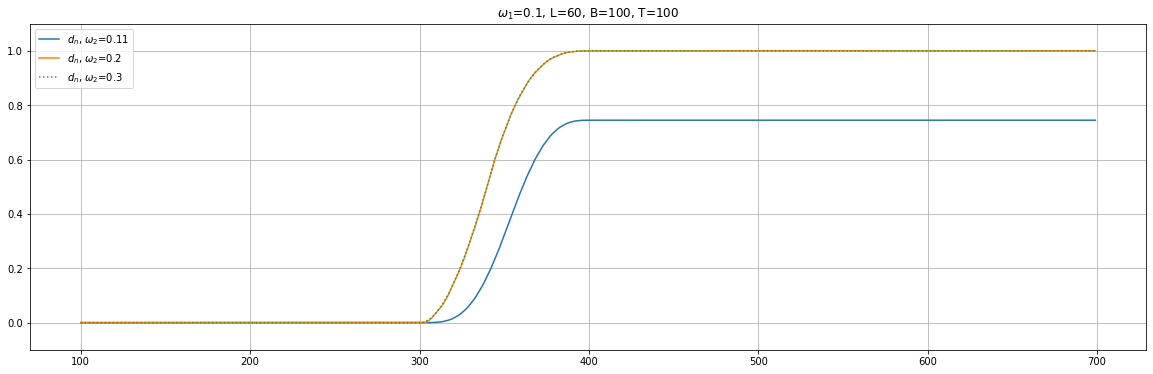
\includegraphics[width=\linewidth]{imgs/diff_omega_growth}
		\end{figure}
		
	\end{frame}
	
	\begin{frame}
		\frametitle{Оценка $ \gamma $: верхняя граница}
		Добавим еще $ 2 $ параметра, подаваемых на вход системе:
		\begin{itemize}
			\item $ \omega_1 $ --- начальная частота ряда;
			\item $ \omega_{min} = \omega_1 + \Delta_{min} $, где $ \Delta_{min} $ --- минимальное для обнаружения неоднородности отклонение частоты ряда от $ \omega_1 $;
		\end{itemize}
		
		Таким образом, имея значение $ g(\omega_1, \omega_{min}) $, для определения порога $ \gamma $, мы можем попытаться аппроксимировать переходный интервал функции обнаружения $ d_n $. 
		
		Обозначим эту аппроксимацию $ a_T $.
		
	\end{frame}
	

	\begin{frame}
		\frametitle{Предпосылки: переходный интервал}
		Матрица $ \mathbb{X} $ имеет размерность $ L \times K $. Рассмотрим траекторные матрицы $ \mathbb{X}_{test}^{(j)} $ размерности $ L \times K_{test} $ тестовых рядов $ F_{j, j+T} $, где $ K_{test} = T - L + 1 $, $ j \in [0, N-T) $. 
		
		$ \forall \; j \in [0, Q - T), \forall \; n \in [1, K_{test}]: \mathrm{X}_n \in \mathbb{X}_{test}^{(j)},  \mathrm{X}_n \in \mathfrak{L}_r^{(1)}$.
		
		$ \forall \; j \in [Q+T, N-T), \forall \; n \in [1, K_{test}]: \mathrm{X}_n \in \mathbb{X}_{test},  \mathrm{X}_n \notin \mathfrak{L}_r^{(1)} $. 
		
		\bigskip
		
		При $ T > 2 \cdot L $, $ \forall \; j \in [Q - T + L, Q - L)$, $ X_{test}^{(j)} $ состоит из:
		
		\begin{itemize}
			\item $ n_B = n_B(j) $ векторов вложений, лежащих в $ \mathfrak{L}_r^{(1)} $;
			\item $ n_Q = n_Q(j) $ векторов вложений, содержащих момент возмущения;
			\item $ n_A = n_A(j) $ векторов вложений, содержащих только значения ряда после разладки.
		\end{itemize}
		
		Причем $ K_{test} = n_B + n_Q + n_A $
		
	\end{frame}

	\begin{frame}
		\frametitle{Предпосылки: переходный интервал}
		Пусть $ L $ --- фиксировано. 
		\tiny
		$$ 1 - \frac{\sum\limits_{l=1}^{K_{test}}\;\sum\limits_{i=1}^{r}\langle X_l, U_i^{(1)}\rangle^2}{\sum\limits_{l=1}^{K_{test}}\|X_l\|^2} = $$
		$$ = 1 - \frac{\sum\limits_{l=1}^{n_B}\;\sum\limits_{i=1}^{r}\langle X_l, U_i^{(1)}\rangle^2 + \sum\limits_{l=n_B}^{n_B + n_Q}\;\sum\limits_{i=1}^{r}\langle X_l, U_i^{(1)}\rangle^2 + \sum\limits_{l=n_B + n_Q}^{K_{test}}\;\sum\limits_{i=1}^{r}\langle X_l, U_i^{(1)}\rangle^2}{\sum\limits_{l=1}^{n_B}\|X_l\|^2 + \sum\limits_{l=n_B}^{n_B+n_Q}\|X_l\|^2 + \sum\limits_{l=n_B+n_Q}^{K_{test}}\|X_l\|^2} = $$
		$$ = 1 - \frac{0 + \sum\limits_{l=n_B}^{n_B+n_Q}\;\sum\limits_{i=1}^{r}\langle X_l, U_i^{(1)}\rangle^2 + n_A(j) \cdot c_H}{c_1 + \sum\limits_{l=n_B}^{n_B+n_Q}\|X_l\|^2 + c_2} \approx 1 - \frac{n_A(j) \cdot c_H}{c_1 + c_2},$$
		\small
		при $ T \rightarrow \infty $ в силу $ n_Q = o(T) $.
		
		Так как для вычисления $ d_n $ мы последовательно смещаем тестовые ряды на $ 1 $ элемент, $ n_A(j) $ возрастает линейно, начиная c $ j = Q-T+L $, $ n_A(j) = j - Q + T - L $.
		
	\end{frame}
	
	\begin{frame}
		\frametitle{Предпосылки: переходный интервал}
		Аналогично, при уменьшении $ L $ переходный интервал также становится более линейным в силу увеличения $ K_{test}^{(j)} $ и, следовательно, $ n_A(j) $.
		\begin{figure}[b]
			\centering
			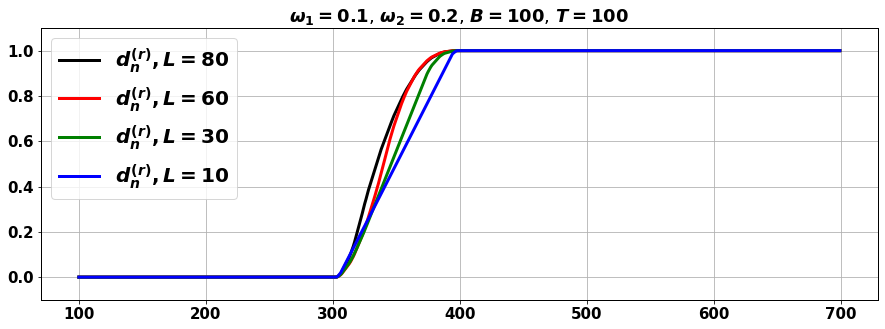
\includegraphics[width=\linewidth]{imgs/row_linear_growth}
		\end{figure}
	\end{frame}
	
	\begin{frame}
		\frametitle{Аппроксимация: Идея}
		Таким образом, мы можем аппроксимировать переходный интервал от $ \gamma_{min} $ до $ g(\omega_1, \omega_{min}) $ прямой $ a_T $. 
		\begin{figure}[b]
			\centering
			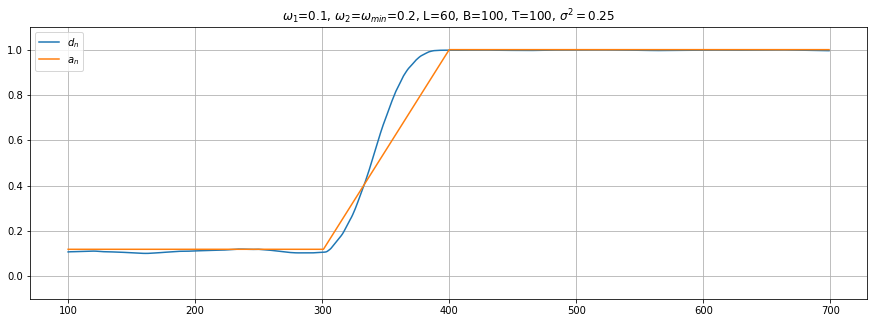
\includegraphics[width=0.6\linewidth]{imgs/row_linear_approximation_1}
		\end{figure}
		
		\begin{figure}[b]
			\centering
			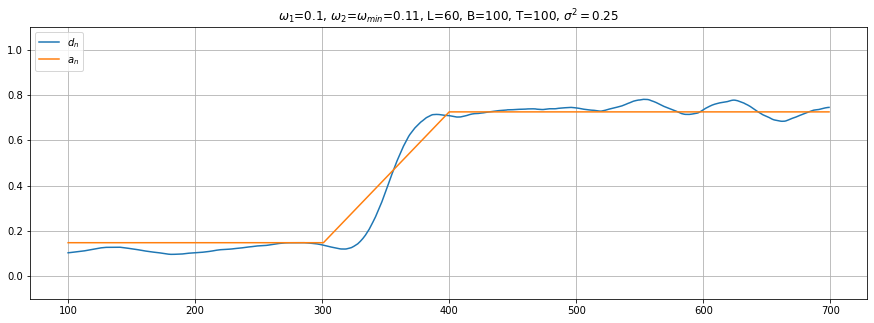
\includegraphics[width=0.6\linewidth]{imgs/row_linear_approximation_2}
		\end{figure}
		\small
		Важно отметить, раз мы хотим брать $ \gamma $ как значение $ a_T $ в точке $ k $, нам важно чтобы начало прямой $ a_T $ было не больше, чем значения $ d_n $ на переходном интервале. Однако такая аппроксимация не всегда корректна.
	\end{frame}
	
	\begin{frame}
		\frametitle{Алгоритм выбора $ \gamma $}
		Таким образом, мы выбраем $ \gamma $ как значение линейной аппроксимации $ a_T $ переходного интервала функции $ d_n $ в точке k.
		
		\bigskip
		Алгоритм:
		\begin{enumerate}
			\item Оцениваем $ \gamma_{min} $;
			\item Вычисляем $ g(\omega_1, \omega_{min}) $;
			\item Строим $ a_T $;
			\item Фиксируем $ \gamma $.
		\end{enumerate}
	\end{frame}

	\begin{frame}
		\frametitle{Алгоритм работы}
		Собирая все вместе, получаем систему:
		\begin{itemize}
			\item Входные данные: $ F_N $, $\omega_1$, $\omega_{min}$, $ k $;
			\item Результат: $\hat{Q}$;
			\item Алгоритм:
			\begin{enumerate}
				\item Оцениваем $ \gamma_{min} $;
				\item Вычисляем $ g(\omega_1, \omega_{min}) $;
				\item Строим $ a_T $;
				\item Фиксируем $ \gamma $.
				\item Определение $ \hat{Q} $ как момент преодоления $ d_n $ значения $ \gamma_a $.
			\end{enumerate}	
		\end{itemize}		
	\end{frame}
	
	
	
	
	\begin{frame}
		\frametitle{Пример работы}
		Зафиксируем параметры: 
		$ \omega_1=\frac{1}{10}, \omega_{min}=\frac{1}{100}, k=30, \omega_2=\frac{1}{5}, Q=301, L=60, B=100, T=100, \sigma^2=0.25 $.
		
		\bigskip
		
		При таких параметрах, для графика ниже $ \gamma_{min}=0.13, \gamma_{max} = 0.725 $,  $ \gamma_a = 0.311$, $ \hat{Q}=326 $.
		\begin{figure}[b]
			\centering
			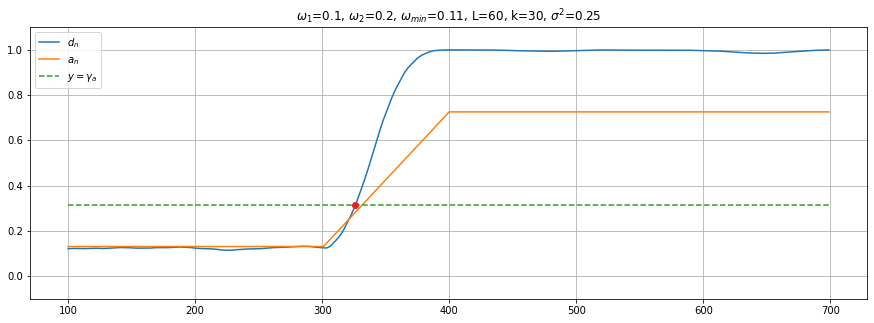
\includegraphics[width=\linewidth]{imgs/example_system_work.png}
		\end{figure}
	\end{frame}
	
	\begin{frame}
		\frametitle{Параметры}
		Все параметры, используемые выше можно разделить на категории: 
		\begin{enumerate}
			\item Входные: $ \omega_1, \omega_{min}, k$;
			\item Зависимые от входных параметров: $ \gamma_{min}, \gamma_{max}, \gamma_a $.
			\item Неизвестные: $ \omega_2, Q $;
			\item Произвольные, выбираемые системой: $ L, B, T $.
			
		\end{enumerate}
		
		Первую категорию параметров можно интерпретировать как заданные пользователем системы. Они фиксированы и не могут меняться для определения более хорошего порога.
		
		\bigskip
		
		Вторая категория зависит от входных параметров и определяется алгоритмом работы.
				
		\bigskip
		
		Третья категория зависит от ряда, подаваемого системе и вообще говоря не известны.
		
		\bigskip
		
		Четвертая категория параметров - те, которые система может подстраивать под тот или иной ряд. Позже попробуем оценить их влияние на оценку системы.
	\end{frame}
	
	
	
	\begin{frame}
		\frametitle{Оценка системы}
		Зафиксируем дисперсию шума $ \sigma^2 = 0.25 $ и введем характеристики системы:
		
		\begin{itemize}
			\item $ FP(\gamma) $ - преодоление порога $ \gamma $ кривой $ d_n $ до момента $ Q $
			\item $ TP(\gamma) $ - преодоление порога $ \gamma $ кривой $ d_n $ в промежутке $ [Q, Q+k] $
		\end{itemize}
		
		Значения параметров рассмотренных категорий оставим такими же. 
		
		\bigskip
		
		Промоделируем реализации шума $ n_{iter} = 200 $ раз и для $ \forall \gamma \in [0, 1] $ с шагом $ 0.01 $ определим $ FPR(\gamma) = \frac{FP}{n_{iter}} $ и $ TPR(\gamma) = \frac{TP}{n_{iter}} $.
		
		Также будем смотреть на $ FPR(\gamma_a) $.
		
	\end{frame}
	
	\begin{frame}
		\frametitle{Оценка системы}
		\begin{figure}[b]
			\centering
			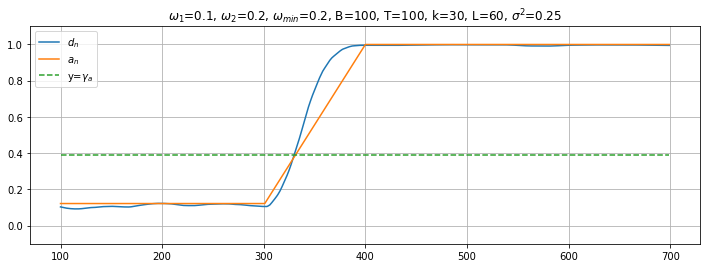
\includegraphics[width=0.85\linewidth]{imgs/system_estimation_one_iter.png}
		\end{figure}
		
		\begin{figure}[b]
			\centering
			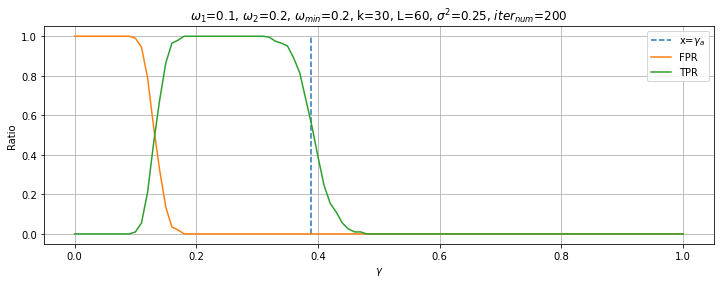
\includegraphics[width=0.85\linewidth]{imgs/system_estimation.png}
		\end{figure}
		
	\end{frame}
	
	
	\begin{frame}
		\frametitle{Оценка влияния параметров: T=70}
		
		\begin{figure}[b]
			\centering
			\subfloat{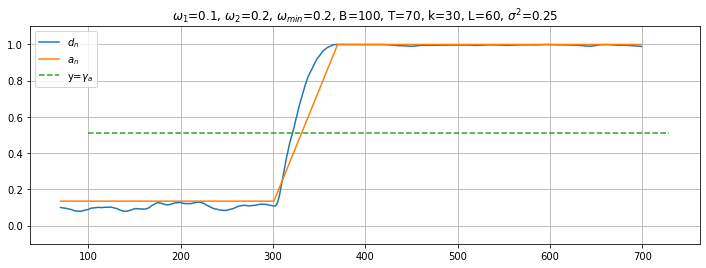
\includegraphics[width=0.85\linewidth]{imgs/system_estimation_one_iter_t=70.png}}
			
			\smallskip
			\subfloat{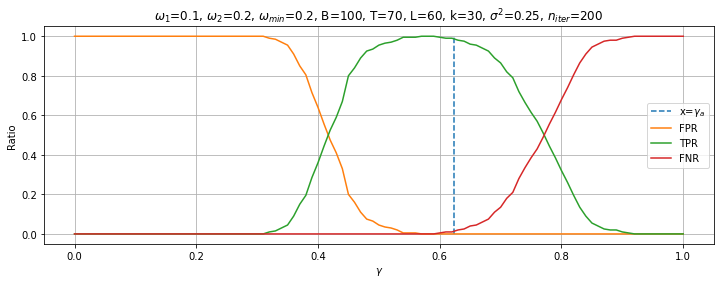
\includegraphics[width=0.85\linewidth]{imgs/system_estimation_t=70.png}}
		\end{figure}
	\end{frame}

	\begin{frame}
		\frametitle{Оценка влияния параметров: T=130}
		
		\begin{figure}[b]
			\centering
			\subfloat{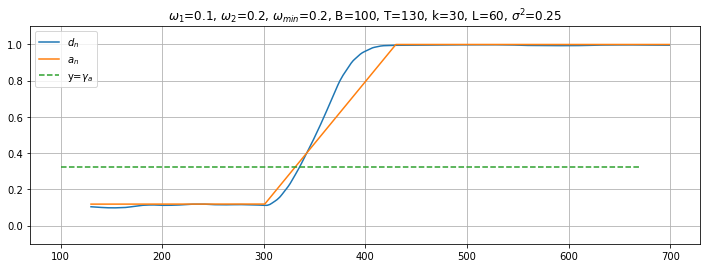
\includegraphics[width=0.65\linewidth]{imgs/system_estimation_one_iter_t=130.png}}
			
			\smallskip
			\subfloat{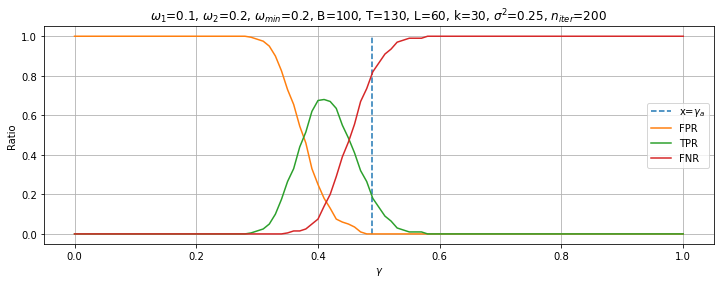
\includegraphics[width=0.65\linewidth]{imgs/system_estimation_t=130.png}}
		\end{figure}
		
		Из изображений видно, что влияя на параметр $ T $ мы можем регулировать скорость возрастания $ d_n $ на переходном интервале и добиться основного требования к $ a_T $ --- значения должны быть не больше чем у $ d_n $.
		
	\end{frame}
	
	\begin{frame}
		\frametitle{Оценка влияния параметров: $ T \approx L $}
		Выше было видно, что уменьшая $ T $, мы можем уменьшить значение $ FPR(\gamma_a) $. Однако при $ T \rightarrow L $, количество элементов в тестовых рядах для подсчета индекса неоднородности $ g $ сокращается, усиливая влияние шума на подсчет элементов $ d_{n} $, что приводит к усилению колебаний и увеличению $ FPR(\gamma_a) $.
		
		\begin{figure}[b]
			\centering
			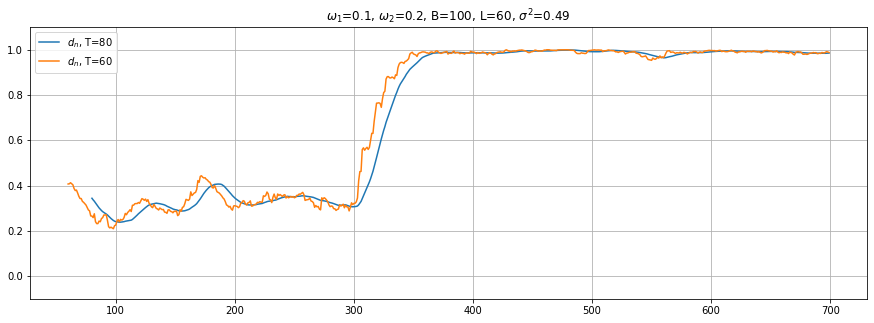
\includegraphics[width=\linewidth]{imgs/decreasing_T.png}
		\end{figure}
	\end{frame}
	
	\begin{frame}
		\frametitle{Оценка влияния параметров: L}
		Как было отмечено ранее, сходимость $ g_a $ и $ g $ достигается при достаточно больших $ L $, однако уменьшая $ L $, переходный интервал $ d_n $ более линеен.
		
		\bigskip
		
		Изменяя параметр $ L $, мы регулируем скорость возрастания кривой $ d_{n} $. Таким образом, подстраивая параметр $ L $ мы можем определять $ \hat{Q} $ раньше момента $ Q + k $.
		
		\begin{figure}[b]
			\centering
			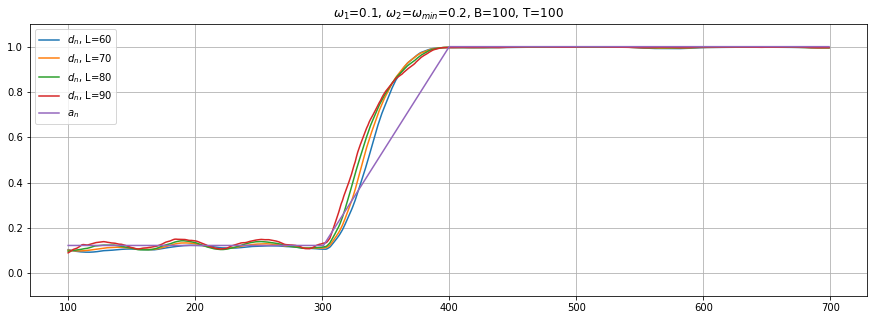
\includegraphics[width=\linewidth]{imgs/row_diff_L.png}
		\end{figure}
		
		
	\end{frame}
	
	\begin{frame}
		\frametitle{Оценка влияния параметров: B}
		В целом, параметр $ B $ не влияет на устойчивость системы в силу предположении о наличии исторических данных и отсутствия влияния на переходный интервал $ d_n $.
		
		\begin{figure}[b]
			\centering
			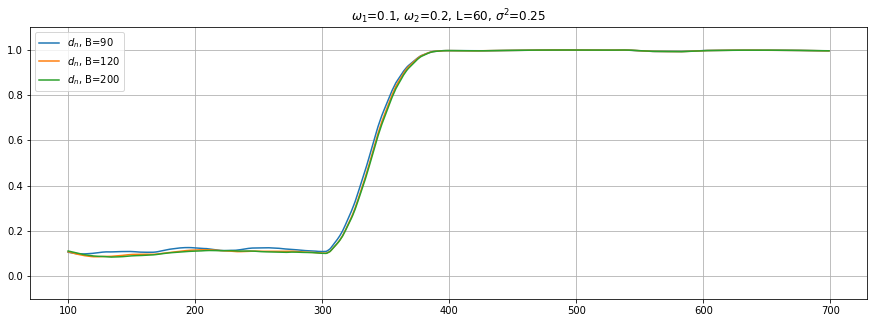
\includegraphics[width=\linewidth]{imgs/row_diff_B.png}
		\end{figure}
		
	\end{frame}
	
	
	\begin{frame}
		\frametitle{Дальнейшие планы}
		\begin{enumerate}
			
			\item 
			Исследовать применимость описанной системы.
		\end{enumerate}
		
	\end{frame}
	
	
	\begin{frame}
		\frametitle{Литература:}
		\begin{thebibliography}{1}
			\bibitem{TSStructure}
			Golyandina, N., Nekrutkin, V., \& Zhigljavsky, A. (2001). Analysis of time series structure: SSA and related techniques. Chapman \& Hall/CRC.
			
		\end{thebibliography}
	\end{frame}
\end{document}